\documentclass{article}

\usepackage[utf8]{inputenc}
\usepackage{algpseudocode}
\usepackage{amsfonts}
\usepackage{amsmath}
\usepackage{bm}
\usepackage{booktabs}
\usepackage{caption}
\usepackage{color}
\usepackage{commath}
\usepackage{empheq}
\usepackage{epsfig}
\usepackage{framed}
\usepackage{graphicx}
\usepackage{grffile}
\usepackage{listings}
\usepackage{mathtools}
\usepackage{pdfpages}
\usepackage{pgfplots}
\usepackage{siunitx}
\usepackage{wrapfig}

% Command "alignedbox{}{}" for a box within an align environment
% Source: http://www.latex-community.org/forum/viewtopic.php?f=46&t=8144
\newlength\dlf  % Define a new measure, dlf
\newcommand\alignedbox[2]{
% Argument #1 = before & if there were no box (lhs)
% Argument #2 = after & if there were no box (rhs)
&  % Alignment sign of the line
{
\settowidth\dlf{$\displaystyle #1$}
    % The width of \dlf is the width of the lhs, with a displaystyle font
\addtolength\dlf{\fboxsep+\fboxrule}
    % Add to it the distance to the box, and the width of the line of the box
\hspace{-\dlf}
    % Move everything dlf units to the left, so that & #1 #2 is aligned under #1 & #2
\boxed{#1 #2}
    % Put a box around lhs and rhs
}
}
% Default fixed font does not support bold face
\DeclareFixedFont{\ttb}{T1}{txtt}{bx}{n}{12} % for bold
\DeclareFixedFont{\ttm}{T1}{txtt}{m}{n}{12}  % for normal
\DeclareMathOperator{\atantwo}{atan2}
\DeclareMathOperator{\acos}{acos}

\def\du#1{\underline{\underline{#1}}}

\definecolor{codegreen}{rgb}{0,0.6,0}
\definecolor{codegray}{rgb}{0.5,0.5,0.5}
\definecolor{codepurple}{rgb}{0.58,0,0.82}
\definecolor{backcolour}{rgb}{0.95,0.95,0.92}

\lstdefinestyle{mystyle}{
    backgroundcolor=\color{backcolour},
    commentstyle=\color{codegreen},
    keywordstyle=\color{magenta},
    numberstyle=\tiny\color{codegray},
    stringstyle=\color{codepurple},
    basicstyle=\footnotesize,
    breakatwhitespace=false,
    breaklines=true,
    captionpos=b,
    keepspaces=true,
    numbers=left,
    numbersep=5pt,
    showspaces=false,
    showstringspaces=false,
    showtabs=false,
    tabsize=2
}

\lstset{style=mystyle}

\author{John Karasinski}
\title{Space Station Remote Manipulator System (SSRMS) Kinematics}

\begin{document}
\maketitle
\tableofcontents
\clearpage

\section{Introduction}

\begin{figure}[b!]
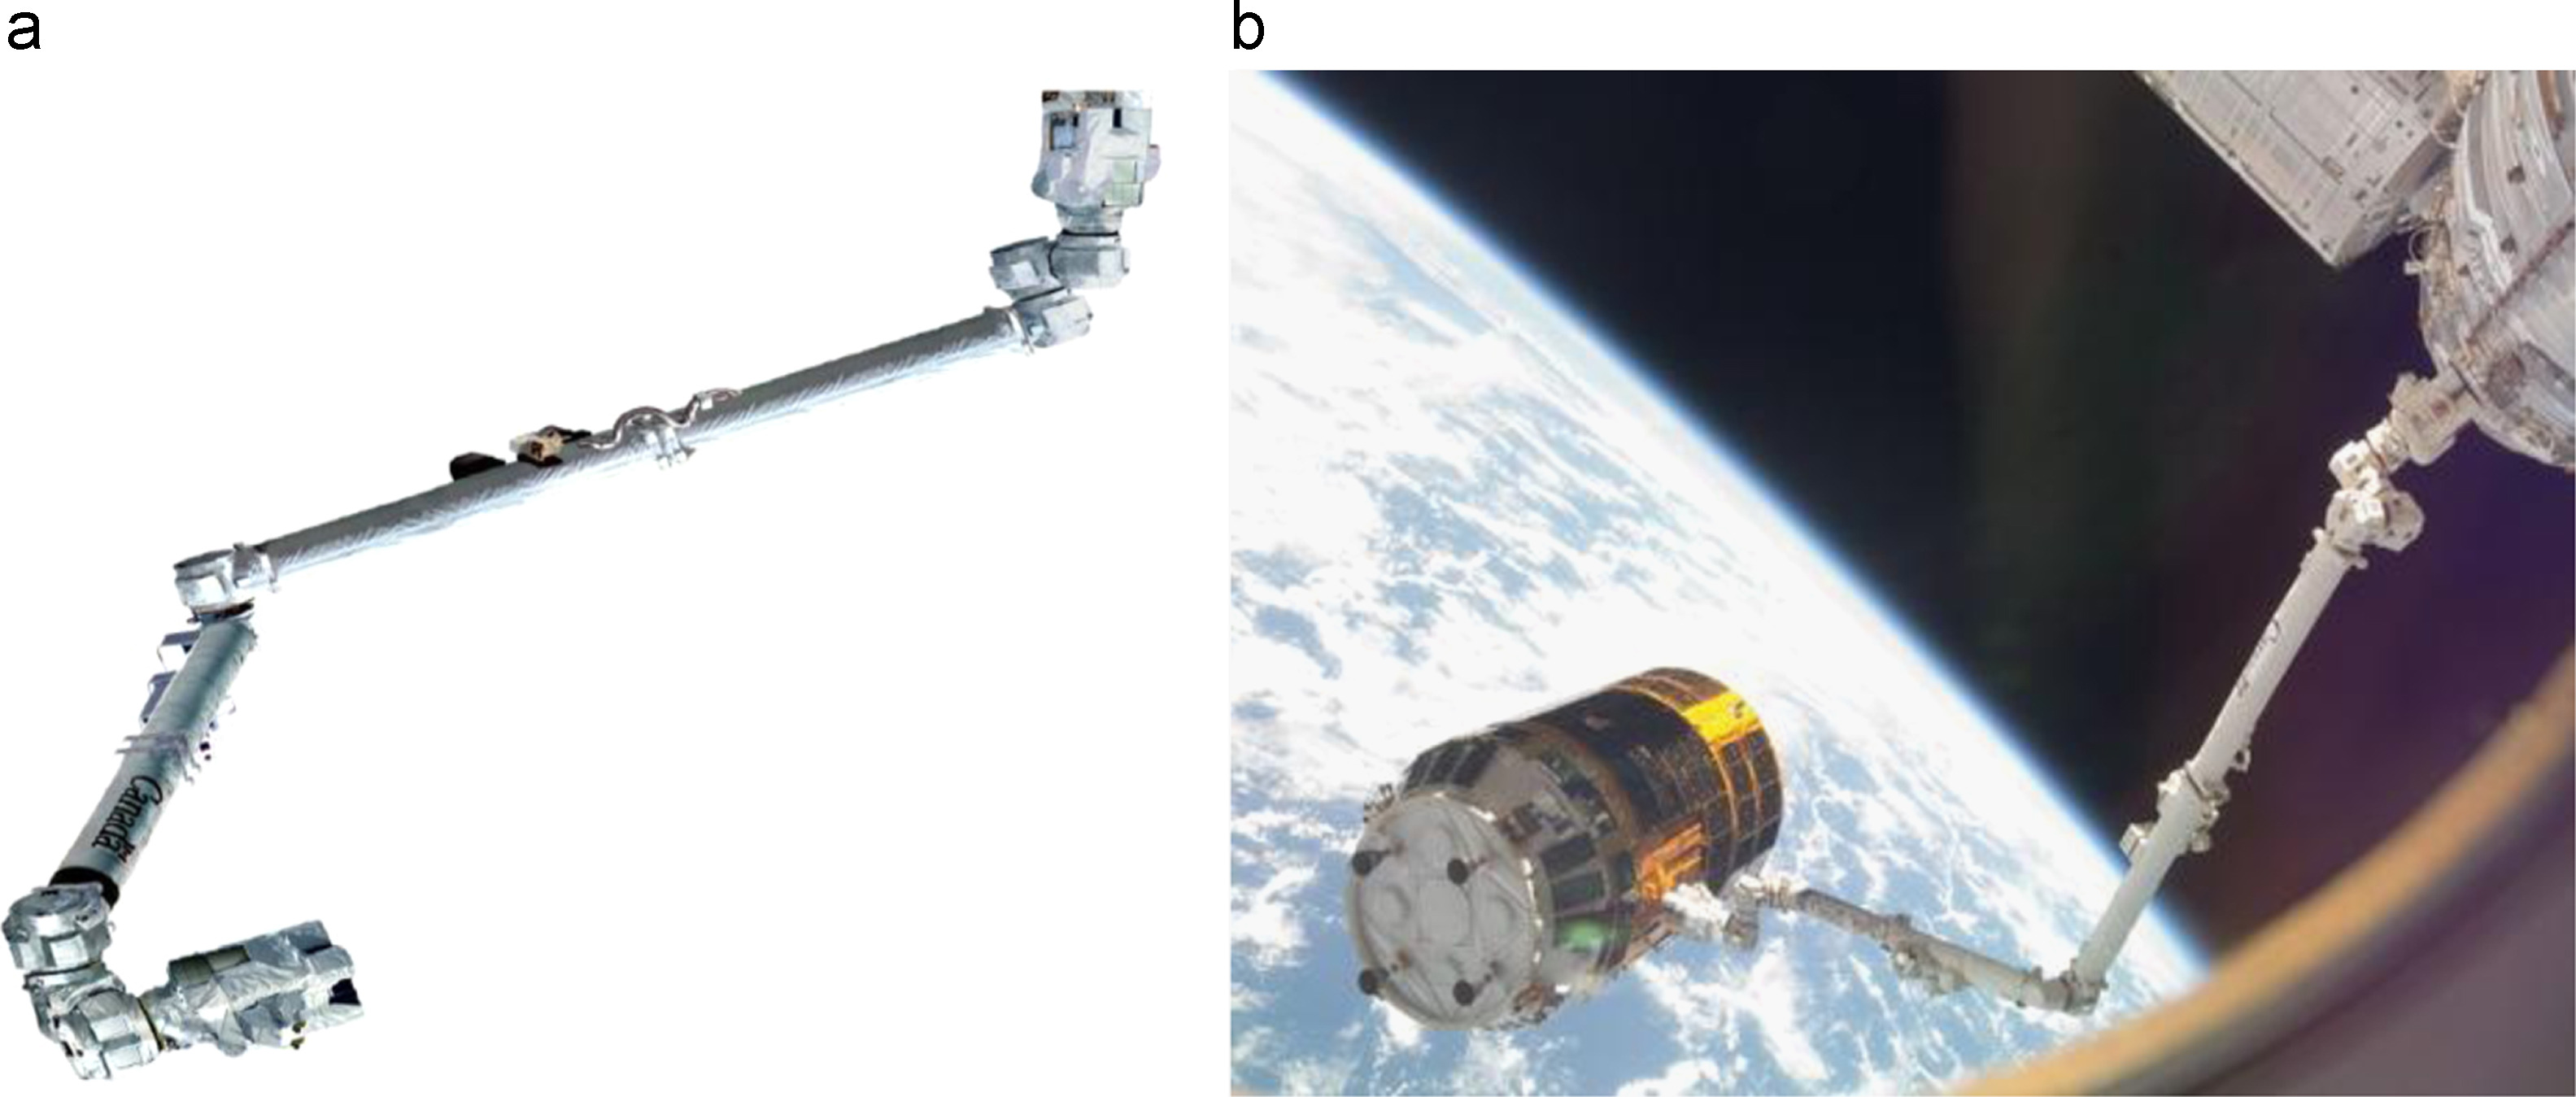
\includegraphics[width=\textwidth]{ssrms.jpg}
\caption{Orbital ATK's Cygnus cargo spacecraft is captured using the Canadarm2 robotic arm on the International Space Station~\cite{ssrms_cc}.}
\label{ssrms_image}
\end{figure}

The Space Station Remote Manipulator System (SSRMS) was designed and built to construct the International Space Station (ISS) and grapple with visiting space vehicles.
The SSRMS is a seven degree of freedom (DoF) manipulator consisting entirely of revolute joints.
The arm is symmetric, consisting of a 3DoF (roll, yaw, pitch) ``shoulder'', an "elbow" pitch joint, and a 3DoF (pitch, yaw, roll) ``wrist''.
Due to this symmetric structure, the arm has the ability to ``walk'' along the station, greatly increasing it's available working space.
The arm can lock the wrist to a grapple fixture, then disconnect the shoulder (which becomes the new wrist) to walk along the station.
See Figure~\ref{ssrms_image} for a picture of the arm grappling a visiting Cygnus vehicle.

The SSRMS is operating from one of the two Robotic Work Stations (RWS) located in either the Cupola or the Destiny module on the ISS.
While operating the arm from the RWS, astronauts commonly lock one of the shoulder joints, which allows for more predictable movement of the arm.
The shoulder roll is the most commonly locked joint during training and operation of the arm~\cite{astro_emails}.
For this reason, we will consider the shoulder roll joint (the first joint of the arm) to be locked at a fixed angle for the majority of this report.

\section{Finite Kinematic Analysis}
\subsection{Denavit-Hartenberg Parameters}
\begin{figure}[b!]
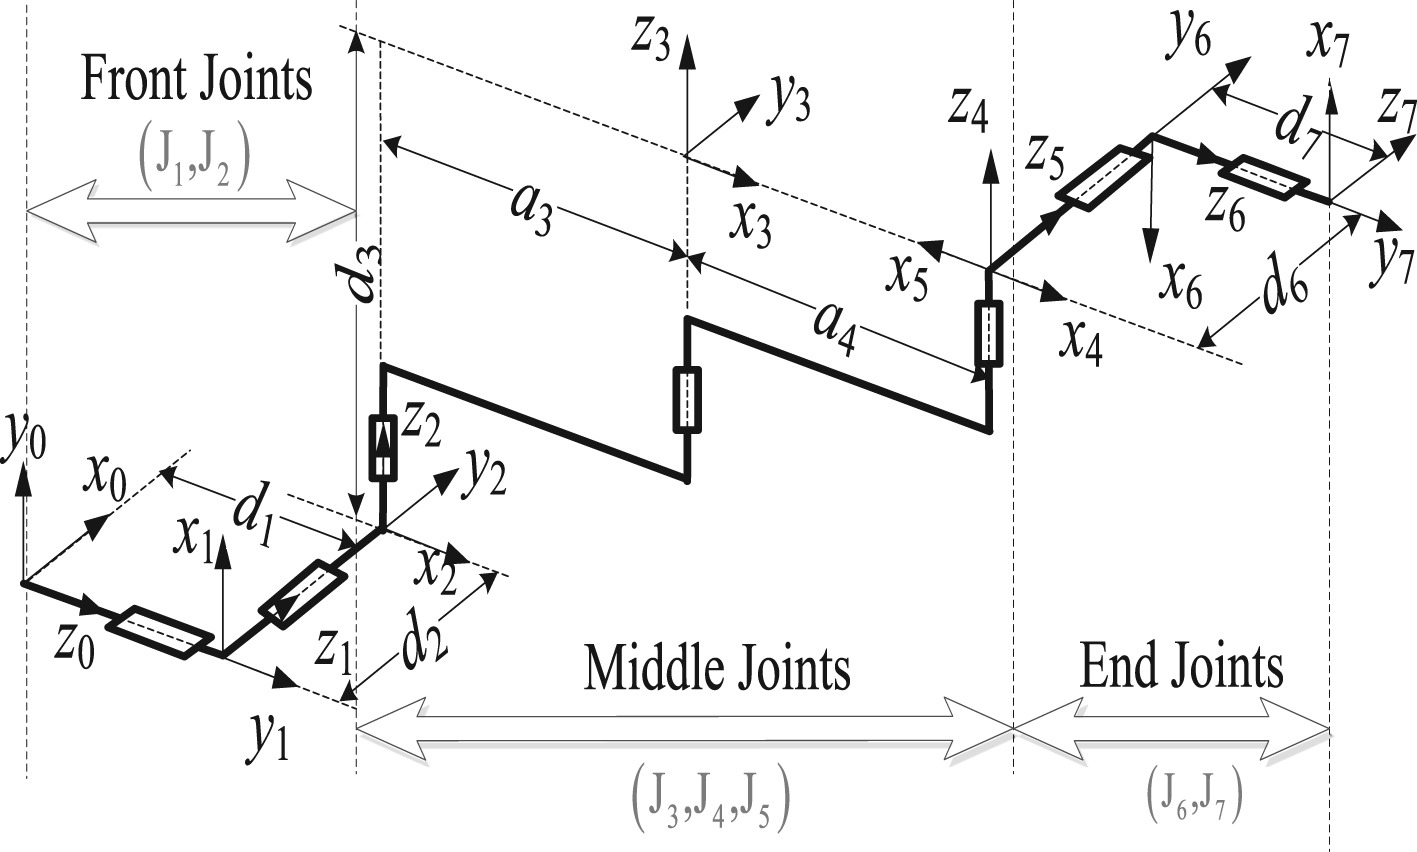
\includegraphics[width=\textwidth]{dh.jpg}
\caption{The Denavit-Hartenberg (D-H) parameters for the Space Station Remote Manipulator System (SSRMS).}
\label{dh_params}
\end{figure}

The Denavit-Hartenberg parameters form a minimal representation of a kinematic linkage of a robotic arm.
These four parameters are the joint angle, $\theta$, the link twist angle, $\alpha$, the link length, $a$, and the joint offset, $d$.
These parameters are identified by inspection, and are based off the coordinates from and lengths defined in Figure~\ref{dh_params}.
The resulting D-H parameters are presented in Table~\ref{dhparams}.
The parameters are plugged into the generic D-H transformation matrix, see Equation~\ref{dh_matrix}.
This equation transforms positions and rotations from the $i^{th}$ to the $i+1^{th}$ coordinates frames.
\begin{align}
T_{i, i+1} &=
\left[\begin{matrix}
\cos{\left (\phi \right )} & - \cos{\left (\alpha \right )} \sin{\left (\phi \right )} &   \sin{\left (\alpha \right )} \sin{\left (\phi \right )} & a \cos{\left (\phi \right )}\\
\sin{\left (\phi \right )} &   \cos{\left (\alpha \right )} \cos{\left (\phi \right )} & - \sin{\left (\alpha \right )} \cos{\left (\phi \right )} & a \sin{\left (\phi \right )}\\
                         0 &   \sin{\left (\alpha \right )}                            &   \cos{\left (\alpha \right )} & d\\
0 & 0 & 0 & 1
\end{matrix}\right]
\label{dh_matrix}
\end{align}

\begin{table}[h]
\centering
\begin{tabular}{c|*{4}{c}}
\toprule
$i$ & $\theta_i$ & $\alpha_i$ & $a_i$ & $d_i$ \\
\midrule
1 &  90 & 90 &     0 & $d_1$ \\
2 &  90 & 90 &     0 & $d_2$ \\
3 &   0 &  0 & $a_3$ & $d_3$ \\
4 &   0 &  0 & $a_4$ &     0 \\
5 & 180 & 90 &     0 &     0 \\
6 & -90 & 90 &     0 & $d_6$ \\
7 & 180 & 90 &     0 & $d_7$ \\
\bottomrule
\end{tabular}
\caption{The Denavit-Hartenberg parameters for the SSRMS. These parameters are the joint angle, $\theta$, the link twist angle, $\alpha$, the link length, $a$, and the joint offset, $d$. These $\theta_i$s give the initial or ``zero-displacement" configuration, but each $\theta_i$ is modeled as an individual variable below.}
\label{dhparams}
\end{table}

The resulting seven matrices are therefore
\begin{align*}
T_{01} &=
\left[\begin{matrix}\cos{\left (\theta_{1} \right )} & 0 & \sin{\left (\theta_{1} \right )} & 0\\\sin{\left (\theta_{1} \right )} & 0 & - \cos{\left (\theta_{1} \right )} & 0\\0 & 1 & 0 & d_{1}\\0 & 0 & 0 & 1\end{matrix}\right]
&&T_{12} =
\left[\begin{matrix}\cos{\left (\theta_{2} \right )} & 0 & \sin{\left (\theta_{2} \right )} & 0\\\sin{\left (\theta_{2} \right )} & 0 & - \cos{\left (\theta_{2} \right )} & 0\\0 & 1 & 0 & d_{2}\\0 & 0 & 0 & 1\end{matrix}\right] \\
T_{23} &=
\left[\begin{matrix}\cos{\left (\theta_{3} \right )} & - \sin{\left (\theta_{3} \right )} & 0 & a_{3} \cos{\left (\theta_{3} \right )}\\\sin{\left (\theta_{3} \right )} & \cos{\left (\theta_{3} \right )} & 0 & a_{3} \sin{\left (\theta_{3} \right )}\\0 & 0 & 1 & d_{3}\\0 & 0 & 0 & 1\end{matrix}\right]
&&T_{34} =
\left[\begin{matrix}\cos{\left (\theta_{4} \right )} & - \sin{\left (\theta_{4} \right )} & 0 & a_{4} \cos{\left (\theta_{4} \right )}\\\sin{\left (\theta_{4} \right )} & \cos{\left (\theta_{4} \right )} & 0 & a_{4} \sin{\left (\theta_{4} \right )}\\0 & 0 & 1 & 0\\0 & 0 & 0 & 1\end{matrix}\right] \\
T_{45} &=
\left[\begin{matrix}\cos{\left (\theta_{5} \right )} & 0 & \sin{\left (\theta_{5} \right )} & 0\\\sin{\left (\theta_{5} \right )} & 0 & - \cos{\left (\theta_{5} \right )} & 0\\0 & 1 & 0 & 0\\0 & 0 & 0 & 1\end{matrix}\right]
&&T_{56} =
\left[\begin{matrix}\cos{\left (\theta_{6} \right )} & 0 & \sin{\left (\theta_{6} \right )} & 0\\\sin{\left (\theta_{6} \right )} & 0 & - \cos{\left (\theta_{6} \right )} & 0\\0 & 1 & 0 & d_{6}\\0 & 0 & 0 & 1\end{matrix}\right] \\
T_{67} &=
\left[\begin{matrix}\cos{\left (\theta_{7} \right )} & 0 & \sin{\left (\theta_{7} \right )} & 0\\\sin{\left (\theta_{7} \right )} & 0 & - \cos{\left (\theta_{7} \right )} & 0\\0 & 1 & 0 & d_{7}\\0 & 0 & 0 & 1\end{matrix}\right]
\end{align*}

Once these seven matrices are defined, it is often desirable to be able to translate directly from the initial coordinate frame to the final end effector frame.
This is easily found by multiplying the successive matrices together to form $T_{07}$, see Equation~\ref{direct}.
Multiplying these matrices together yields
\begin{align}
T_{07} =& T_{01} T_{12} T_{23} T_{34} T_{45} T_{56} T_{67} \label{direct} \\
T_{07}[1, 1] =& \left(- s_{1} c_{345} + s_{345} c_{1} c_{2}\right) s_{7} + \left(s_{1} s_{345} c_{6} + s_{2} s_{6} c_{1} + c_{1} c_{2} c_{6} c_{345}\right) c_{7} \nonumber \\
T_{07}[1, 2] =& s_{1} s_{6} s_{345} - s_{2} c_{1} c_{6} + s_{6} c_{1} c_{2} c_{345} \nonumber \\
T_{07}[1, 3] =& \left(s_{1} c_{345} - s_{345} c_{1} c_{2}\right) c_{7} + \left(s_{1} s_{345} c_{6} + s_{2} s_{6} c_{1} + c_{1} c_{2} c_{6} c_{345}\right) s_{7} \nonumber \\
T_{07}[1, 4] =& a_{3} s_{1} s_{3} + a_{3} c_{1} c_{2} c_{3} + a_{4} s_{1} s_{34} + a_{4} c_{1} c_{2} c_{34} + d_{2} s_{1} + d_{3} s_{2} c_{1} - d_{6} s_{1} c_{345} + d_{6} s_{345} c_{1} c_{2} \nonumber \\
              & + d_{7} s_{1} s_{6} s_{345} - d_{7} s_{2} c_{1} c_{6} + d_{7} s_{6} c_{1} c_{2} c_{345} \nonumber \\
T_{07}[2, 1] =& \left(s_{1} s_{345} c_{2} + c_{1} c_{345}\right) s_{7} + \left(s_{1} s_{2} s_{6} + s_{1} c_{2} c_{6} c_{345} - s_{345} c_{1} c_{6}\right) c_{7} \nonumber \\
T_{07}[2, 2] =& - s_{1} s_{2} c_{6} + s_{1} s_{6} c_{2} c_{345} - s_{6} s_{345} c_{1} \nonumber \\
T_{07}[2, 3] =& - \left(s_{1} s_{345} c_{2} + c_{1} c_{345}\right) c_{7} + \left(s_{1} s_{2} s_{6} + s_{1} c_{2} c_{6} c_{345} - s_{345} c_{1} c_{6}\right) s_{7} \nonumber \\
T_{07}[2, 4] =& a_{3} s_{1} c_{2} c_{3} - a_{3} s_{3} c_{1} + a_{4} s_{1} c_{2} c_{34} - a_{4} s_{34} c_{1} - d_{2} c_{1} + d_{3} s_{1} s_{2} + d_{6} s_{1} s_{345} c_{2} + d_{6} c_{1} c_{345} \nonumber \\
              & - d_{7} s_{1} s_{2} c_{6} + d_{7} s_{1} s_{6} c_{2} c_{345} - d_{7} s_{6} s_{345} c_{1} \nonumber \\
T_{07}[3, 1] =& \left(s_{2} c_{6} c_{345} - s_{6} c_{2}\right) c_{7} + s_{2} s_{7} s_{345} \nonumber \\
T_{07}[3, 2] =& s_{2} s_{6} c_{345} + c_{2} c_{6} \nonumber \\
T_{07}[3, 3] =& \left(s_{2} c_{6} c_{345} - s_{6} c_{2}\right) s_{7} - s_{2} s_{345} c_{7} \nonumber \\
T_{07}[3, 4] =& a_{3} s_{2} c_{3} + a_{4} s_{2} c_{34} + d_{1} - d_{3} c_{2} + d_{6} s_{2} s_{345} + d_{7} s_{2} s_{6} c_{345} + d_{7} c_{2} c_{6} \nonumber \\
T_{07}[4, 1] =& 0 \nonumber \\
T_{07}[4, 2] =& 0 \nonumber \\
T_{07}[4, 3] =& 0 \nonumber \\
T_{07}[4, 4] =& 1 \nonumber
\end{align}

\subsection{Joint/Shape Matrices}
We can similarly use joint and shape matrices to arrive at these $T$ matrices.
Shape matrices allow for a more general approach compared to D-H matrices, and ``avoid the difficulties that sometimes arise in the use of D-H matrices''~\cite{uicker2013matrix}.
For simplicity of readability, we renumber the joints from $1-7$ to $A-G$.
All of the joints of the SSRMS are revolute.
A general revolute joint, $h$, can be modeled with the joint matrix of
\begin{align*}
\Phi_h \left( \phi_h \right) =
\left[\begin{matrix}
\cos \phi_h & -\sin \phi_h & 0 & 0 \\
\sin \phi_h & \cos \phi_h & 0 & 0 \\
0 & 0 & 1 & 0 \\
0 & 0 & 0 & 1
\end{matrix}\right]
\end{align*}
\begin{align}
T_{i,i+1} &= S_{i, j} J_j S_{i+1,j}^{-1} \label{joint_eq} \\
T_{01} &= S_{0A} J_A S_{1A}^{-1} \nonumber \\
T_{12} &= S_{1B} J_B S_{2B}^{-1} \nonumber \\
T_{23} &= S_{2C} J_C S_{3C}^{-1} \nonumber \\
T_{34} &= S_{3D} J_D S_{4D}^{-1} \nonumber \\
T_{45} &= S_{4E} J_E S_{5E}^{-1} \nonumber \\
T_{56} &= S_{5F} J_F S_{6F}^{-1} \nonumber \\
T_{67} &= S_{6G} J_G S_{7G}^{-1} \nonumber
\end{align}
For joints $J_A, J_B, J_C, J_D, J_E, J_F,$ and $J_G$, we also define two shape matrices.
\begin{align*}
\phantom{T_{01}}&%=
% \begin{bmatrix*}[c]
%  1 & 0 & 0 & x_0 \\
%  0 & 1 & 0 & y_0 \\
%  0 & 0 & 1 & z_0 \\
%  0 & 0 & 0 & 1 \\
% \end{bmatrix*},
&& S_{0A} = I,
S_{1A} =
\begin{bmatrix*}[c]
1 & 0 & 0 & 0 \\
0 & 0 & 1 & -d_1 \\
0 & -1 & 0 & 0 \\
0 & 0 & 0 & 1 \\
\end{bmatrix*}, \\
S_{1B} &= I,
S_{2B} =
\begin{bmatrix*}[c]
1 & 0 & 0 & 0 \\
0 & 0 & 1 & -d_2 \\
0 & -1 & 0 & 0 \\
0 & 0 & 0 & 1 \\
\end{bmatrix*},
&& S_{2C} = I,
S_{3C} =
\begin{bmatrix*}[c]
1 & 0 & 0 & -a_3 \\
0 & 0 & 1 & -d_3 \\
0 & 1 & 0 & 0 \\
0 & 0 & 0 & 1 \\
\end{bmatrix*}, \\
S_{3D} &= I,
S_{4D} =
\begin{bmatrix*}[c]
1 & 0 & 0 & -a_3 \\
0 & 0 & 1 & 0 \\
0 & 1 & 0 & 0 \\
0 & 0 & 0 & 1 \\
\end{bmatrix*},
&& S_{4E} = I,
S_{5E} =
\begin{bmatrix*}[c]
1 & 0 & 0 & 0 \\
0 & 0 & 1 & 0 \\
0 & -1 & 0 & 0 \\
0 & 0 & 0 & 1 \\
\end{bmatrix*}, \\
S_{5F} &= I,
S_{6F} =
\begin{bmatrix*}[c]
1 & 0 & 0 & 0 \\
0 & 0 & 1 & -d_6 \\
0 & -1 & 0 & 0 \\
0 & 0 & 0 & 1 \\
\end{bmatrix*},
&& S_{6G} = I,
S_{7G} =
\begin{bmatrix*}[c]
1 & 0 & 0 & 0 \\
0 & 0 & 1 & -d_7 \\
0 & -1 & 0 & 0 \\
0 & 0 & 0 & 1 \\
\end{bmatrix*}
\end{align*}
Multiplying out these shape and joint matrices according toe Equation~\ref{joint_eq} yields the same $T$ matrices as obtained using the Denavit-Hartenberg parameters.

\subsection{Inverse Kinematics}
\subsubsection{Method}
The SSRMS has eight solutions of joint angles for any such given pose~\cite{xu2014analytical}.
In their 2014 paper, Xu et al. show how to to solve for these configurations using a series of flags labeled ``SHOULDER'', ``WRIST'', and ``ELBOW''.
After locking the first rotary joint at a known angle, there are a pair of solutions for the second joint known as the ``SHOULDER'' configuration.
With the first two joints known, it is then possible to solve for the final two joints, giving the ``WRIST'' configuration.
Finally, the middle three joints can be solved for, giving the ``ELBOW'' configuration.

This technique was inspired by a 1984 paper by Lee and Ziegler which used this geometric approach to solve for the inverse kinematics of PUMA robots~\cite{lee1984geometric}.
In their paper, Lee and Ziegler define 4 ``indicators'' (``ARM'', ``ELBOW'', ``WRIST'', and `FLIP'') based off the geometric configuration of the PUMA robot.
These indicators were used to provide consistent solutions for the PUMA robots during movement through their workspace.
Lee and Ziegler presented an algorithmic approach which was programmed to show how their method could be used in practice.
An example of two of these indicators in shown in Figure~\ref{puma}.

For the SSRMS solution presented below, the SHOULDER, ELBOW, and WRIST configuration indicators take on the follow values~\cite{xu2014analytical}
\begin{align*}
\text{SHOULDER}&=\begin{cases}
	+1, & \text{right shoulder}.\\
	-1, & \text{left shoulder}.
\end{cases}\\
\text{ELBOW}&=\begin{cases}
	+1, & \text{outside elbow}.\\
	-1, & \text{inside elbow}.
\end{cases}\\
\text{WRIST}&=\begin{cases}
	+1, & \text{wrist down}.\\
	-1, & \text{wrist up}.
\end{cases}
\end{align*}

\begin{figure}[b!]
\begin{centering}
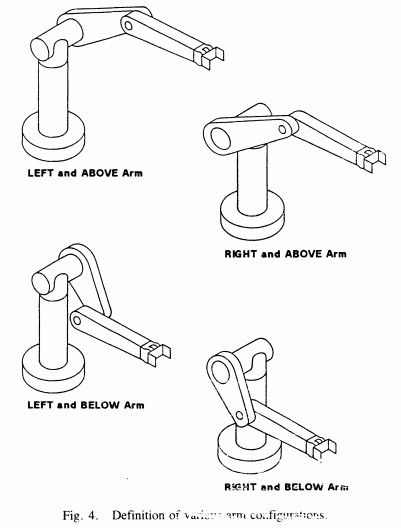
\includegraphics[width=0.5\textwidth]{puma.jpg}
\caption{Definition of two of the PUMA robotic arm configurations, taken from Lee and Ziegler~\cite{lee1984geometric}.}
\label{puma}
\end{centering}
\end{figure}

\subsubsection{SSRMS Solution}
In general, for a known end effector pose, we can define~\cite{mae225_notes}
\begin{align*}
T_{07} &=
\left[\begin{matrix}
u_x & v_x & w_x & p_x \\
u_y & v_y & w_y & p_y \\
u_z & v_z & w_z & p_z \\
  0 &   0 &   0 &   1 \\
\end{matrix}\right]\\
&= T_{01} T_{12} T_{23} T_{34} T_{45} T_{56} T_{67}
\end{align*}
Premultiplying both sides by $T_{01}^{-1}$ yields,
\begin{align*}
T_{01}^{-1} T_{07} = T_{12} T_{23} T_{34} T_{45} T_{56} T_{67}
\end{align*}
Equating each element $(i,j)$ on both the left and right hand sides yields:
\begin{align}
u_x c_1 + u_y s_1 &= \left(s_{2} s_{6} + c_{2} c_{6} c_{345}\right) c_{7} + s_{7} s_{345} c_{2} \label{eq1} \\
v_x c_1 + v_y s_1 &= - s_{2} c_{6} + s_{6} c_{2} c_{345} \label{eq5} \\
w_x c_1 + w_y s_1 &= \left(s_{2} s_{6} + c_{2} c_{6} c_{345}\right) s_{7} - s_{345} c_{2} c_{7} \label{eq7} \\
p_x c_1 + p_y s_1 &= a_{3} c_{2} c_{3} + a_{4} c_{2} c_{34} + d_{3} s_{2} + d_{6} s_{345} c_{2} - d_{7} s_{2} c_{6} + d_{7} s_{6} c_{2} c_{345} \label{eq3} \\
u_z                 &= \left(s_{2} c_{6} c_{345} - s_{6} c_{2}\right) c_{7} + s_{2} s_{7} s_{345} \label{eq2} \\
v_z                 &= s_{2} s_{6} c_{345} + c_{2} c_{6} \label{eq6} \\
w_z                 &= \left(s_{2} c_{6} c_{345} - s_{6} c_{2}\right) s_{7} - s_{2} s_{345} c_{7} \label{eq8} \\
- d_{1} + p_z       &= a_{3} s_{2} c_{3} + a_{4} s_{2} c_{34} - d_{3} c_{2} + d_{6} s_{2} s_{345} + d_{7} s_{2} s_{6} c_{345} + d_{7} c_{2} c_{6} \label{eq4} \\
u_x s_1 - u_y c_1 &= - s_{7} c_{345} + s_{345} c_{6} c_{7} \label{th51}\\
v_x s_1 - v_y c_1 &= s_{6} s_{345} \label{th53} \\
w_x s_1 - w_y c_1 &= s_{7} s_{345} c_{6} + c_{7} c_{345} \label{th52} \\
p_x s_1 - p_y c_1 &= a_{3} s_{3} + a_{4} s_{34} + d_{2} - d_{6} c_{345} + d_{7} s_{6} s_{345} \\
0                     &= 0 \\
0                     &= 0 \\
0                     &= 0 \\
1                     &= 1
\end{align}
where we have defined $s_i = \sin{i}, c_i = \cos{i}, s_{ij} = \sin{\left(i+j\right)}, c_{ij} = \cos{\left(i+j\right)}, s_{ijk} = \sin{\left(i+j+k\right)}$ and $c_{ijk} = \cos{\left(i+j+k\right)}$.
Manipulating the equations, we take $\left(Eq.~\ref{eq1} \right) s_2 - \left(Eq.~\ref{eq2} \right) c_2$ and simplify, producing
\begin{align}
\left(u_x c_1 + u_y s_1\right) s_2 - u_z c_2 &= s_{6} c_{7} \label{eqc3}
\end{align}
Similarly, we can do $\left(Eq.~\ref{eq3} \right) s_2-\left(Eq.~\ref{eq4}\right) c_2$ and simplify, which results in
\begin{align}
\left(p_x c_1 + p_y s_1 \right) s_2 - \left(- d_{1} + p_z \right) c_2 &= d_3 - c_6 d_7 \label{eqc1}
\end{align}
We can also subtract $\left(Eq.~\ref{eq6} \right) c_2 - \left(Eq.~\ref{eq5} \right) s_2$
\begin{align}
v_z c_2 - \left( v_x c_1 + v_y s_1 \right) s_2 &= c_{6} \label{eqc2}
\end{align}
Finally, we can also subtract $\left(Eq.~\ref{eq7} \right) s_2 - \left(Eq.~\ref{eq8} \right) c_2$
\begin{align}
\left(w_x c_1 + w_y s_1\right) s_2 - w_z c_2 &= s_{6} s_{7} \label{eqc4}
\end{align}
Rearranging Equations~\ref{eqc1} and \ref{eqc2} to be equal to $c_6$ and equating the two yields
\begin{align}
-d_3 &= \left( \left( v_x d_7 - p_x \right) c_1 + \left( v_y d_7 - p_y \right) s_1 \right) s_2 + \left(-v_z d_7 - d_{1} + p_z \right) c_2
\end{align}
Locking the shoulder roll angle to a known angle, $\boxed{\theta_1 = \beta}$, we can solve for $\theta_2$,
\begin{align}
\boxed{\theta_2 = \mbox{SHOULDER} \cdot \acos \left( \dfrac{d_3}{\sqrt{h_1^2 + q_1^2}} \right) + \atantwo(q_1,h_1)}
\end{align}
where
\begin{align}
h_1 &= \left(-v_z d_7 - d_{1} + p_z \right) \\
q_1 &= \left( \left( v_x d_7 - p_x \right) c_{\beta} + \left( v_y d_7 - p_y \right) s_{\beta} \right)
\end{align}
With $\theta_1$ and $\theta_2$ now known, $\theta_6$ can be solved using Equation~\ref{eqc2},
\begin{align}
\boxed{\theta_6 = \mbox{WRIST} \cdot \acos \left(v_z c_2 - \left( v_x c_1 + v_y s_1 \right) s_2 \right)}
\end{align}
And we can then combine Equations~\ref{eqc3} and~\ref{eqc4}, yielding
\begin{align}
\boxed{\theta_7 = \atantwo \left( \dfrac{\left(u_x c_1 + u_y s_1\right) s_2 - u_z c_2}{s_6},
                                  \dfrac{\left(w_x c_1 + w_y s_1\right) s_2 - w_z c_2}{s_6}\right)}
\end{align}
With the shoulder and wrist joints resolved, we can now solve for the middle joints. We now take
\begin{align*}
\left(T_{12}^{-1} \right) \left(T_{17}\right) \left(T_{67}^{-1}\right) \left(T_{56}^{-1}\right) = \left(T_{23}\right) \left(T_{34}\right) \left(T_{45}\right)
\end{align*}
Taking the left and right hand side $\left(1, 4\right)$ and $\left(2, 4 \right)$ elements from the resulting matrix yields
\begin{align}
a_{3} c_{3} + a_{4} c_{34} &= d_{6} \left(w_z s_{2} + c_{2}\left(w_x c_{1} + w_y s_{1}\right) \right) c_{7} \nonumber \\
                           &\phantom{=} - d_{6} \left(u_z s_{2} + c_{2}\left(u_x c_{1} + u_y s_{1} \right) \right) s_{7}  \nonumber \\
                           &\phantom{=} - d_{7} \left(v_z s_{2} + c_{2}\left(v_x c_{1} + v_y s_{1} \right) \right) \nonumber \\
                           &\phantom{=}+ \left(- d_{1} + p_z\right) s_{2} + c_{2}\left(p_x c_{1} + p_y s_{1}\right) \label{mj1} \\
a_{3} s_{3} + a_{4} s_{34} &= - d_{2} + d_{6} \left(w_x s_{1} - w_y c_{1}\right) c_{7} - d_{6} \left(u_x s_{1} - u_y c_{1}\right) s_{7} \nonumber \\
                           &\phantom{=} - d_{7} \left(v_x s_{1} - v_y c_{1}\right) + p_x s_{1} - p_y c_{1} \label{mj2}
\end{align}
$\theta_4$ is then solved by combining the above two equations, resulting in
\begin{align}
\boxed{\theta_4 = \mbox{ELBOW} \cdot \acos \left( \dfrac{X^2 + Y^2 - a_3^2 - a_4^2}{2 a_3 a_4} \right)}
\end{align}
where
\begin{align*}
X &= d_{6} \left( \left(w_z s_{2} + c_{2}\left(w_x c_{1} + w_y s_{1}\right) \right) c_{7} - \left(u_z s_{2} + c_{2}\left(u_x c_{1} + u_y s_{1} \right) \right) s_{7} \right) \nonumber \\
  &\phantom{=}- d_{7} \left(v_z s_{2} + c_{2}\left(v_x c_{1} + v_y s_{1} \right) \right) + \left(- d_{1} + p_z\right) s_{2} + c_{2}\left(p_x c_{1} + p_y s_{1}\right) \\
Y &= - d_{2} + d_{6} \left(w_x s_{1} - w_y c_{1}\right) c_{7} - d_{6} \left(u_x s_{1} - u_y c_{1}\right) s_{7} - d_{7} \left(v_x s_{1} - v_y c_{1}\right) + p_x s_{1} - p_y c_{1}
\end{align*}
Substituting the solution into $\theta_4$ and Equations~\ref{mj1} and~\ref{mj2} and combining yields
\begin{align*}
\boxed{\theta_3 = \atantwo \left(Y \left( a_3 + a_4 c_4 \right) - X a_4 s_4, X \left(a_3 + a_4 c_4 \right) + Y a_4 s_4 \right)}
\end{align*}
Subtracting $(Eq.~\ref{th52}) c_7$ and $(Eq.~\ref{th51}) s_7$ yields
\begin{align*}
c_{345} &= \left(w_x s_1 - w_y c_1\right) c_7 - \left(u_x s_1 - u_y c_1 \right) s_7
\end{align*}
And from Equation~\ref{th53} we have
\begin{align*}
s_{345} = \dfrac{v_x s_1 - v_y c_1 }{s_{6}}
\end{align*}
which we can combine to solve for the last joint
\begin{align*}
\theta_5 &= \left(\theta_3 + \theta_4 + \theta_5 \right) - \left(\theta_3 + \theta_4 \right) \\
\alignedbox{\theta_5}{=\atantwo \left(s_{345}, c_{345} \right) - \left(\theta_3 + \theta_4 \right)}
\end{align*}

\subsection{Numerical Example}
% Tt.subs({theta1: rad(90), theta2: rad(90), theta3: 0, theta4: 0, theta5: rad(180), theta6: rad(-90), theta7: rad(180)}).subs({a3:2.3, a4:2.3, d1:0.65, d2:0.3,d3:0.9,d6:0.3,d7:0.65})
For practical purposes, the link length and offset values can be set to
\begin{align*}
&a_{3} = 2.30, a_{4} = 2.30, d_{1} = 0.65, d_{2} = 0.30 \\
&d_{3} = 0.90, d_{6} = 0.30, d_{7} = 0.65
\end{align*}
As an example, plugging in these values and the initial angles given in Table~\ref{dhparams} into Equation~\ref{direct} yields
\begin{align*}
T_{07} &=
\left[\begin{matrix}
0 & 0 & 1 & 0.6 \\
1 & 0 & 0 & 0.9 \\
0 & 1 & 0 & 5.9 \\
0 & 0 & 0 &   1 \\
\end{matrix}\right] \\
\end{align*}
As another example, given the end effector pose
\begin{align*}
T_{07} &=
\left[\begin{matrix}
0.8021 & 0.1217 & 0.5846 & 2.4790 \\
-0.5859 & 0.3495 & 0.7311 & -2.4734 \\
-0.1154 & 0.9290 & 0.3517 & -0.4927 \\
0 & 0 & 0 & 1
\end{matrix}\right] \\
\end{align*}
and locking the first joint variable $\theta_1 = \beta = 60^\circ$, we can solve for the 8 possible configurations of the arm
\begin{table}[h]
\centering
\begin{tabular}{*{10}{r}}
\toprule
S & E & W & $\theta_1$ & $\theta_2$ & $\theta_3$ & $\theta_4$ & $\theta_5$ & $\theta_6$ & $\theta_7$ \\
\midrule
 1 &  1 &  1 & 60.000 &  -20.268   &  64.074 &   79.722 & -149.770 &  138.205 & -77.426 \\
 1 &  1 & -1 & 60.000 &  -20.268   &  58.153 &   99.444 &   16.428 & -138.205 & 102.573 \\
 1 & -1 &  1 & 60.000 &  -20.268   & 143.797 &  -79.722 &  -70.048 &  138.205 & -77.426 \\
-1 &  1 &  1 & 60.000 & -109.087   &  35.576 &   79.140 & -119.938 &   49.659 & -85.275 \\
 1 & -1 & -1 & 60.000 &  -20.268   & 157.598 &  -99.444 &  115.872 & -138.205 & 102.573 \\
-1 &  1 & -1 & 60.000 & -109.087   &  23.189 &  100.025 &   51.565 &  -49.659 &  94.724 \\
-1 & -1 &  1 & 60.000 & -109.087   & 114.717 &  -79.140 &  -40.797 &   49.659 & -85.275 \\
-1 & -1 & -1 & 60.000 & -109.087   & 123.214 & -100.025 &  151.590 &  -49.659 &  94.724 \\
\bottomrule
\end{tabular}
\caption{The eight possible configurations for locking the first joint, where S, E, and W stand for "SHOULDER", "ELBOW", and "WRIST", respectively.}
% \label{dhparams}
\end{table}

\section{Differential Kinematic Analysis}
\subsection{Method 1: Kinematic Jacobian}
Where $\hat{z}_i$ is taken from the last column of $T_{1i}$, and can be defined
\begin{align*}
T_{1i} &=
\left[\begin{matrix}
  & \du{\Theta}_i &   & \vdots & a_i \\
  & \hdots   &   &        & \hdots \\
0 &        0 & 0 & \vdots & 0
\end{matrix}\right] \\
\du{\Theta}_i &=
\left[\begin{matrix}
& & \\
x_i & y_i & z_i \\
& &
\end{matrix}\right] \\
\hat{z}_i &= \left( \prod_{i=1}^n \du{\Theta}_i \right) z_i
\end{align*}
and $\vec{r}_i$ is defined
\begin{align*}
\vec{r}_i = \sum_{i=1}^n \vec{a}_i
\end{align*}
With these definitions, we can find the Jacobian via
\begin{align*}
\dot{\vec{P}} &= \sum_{i=1}^{n} \left( \hat{z}_i \times \vec{r}_i \right) \dot{\theta}_i \\
\vec{w} &= \sum_{i=1}^{n} \dot{\theta}_i \hat{z}_i \\
\du{J} \dot{q} &=
\left[\begin{matrix}
\underline{\dot{P}} \\
\underline{\vec{w}}
\end{matrix}\right] \\
\left[\begin{matrix}
\hat{z}_1 \times \vec{r}_1 & \hat{z}_2 \times \vec{r}_2 & \cdots & \hat{z}_7 \times \vec{r}_7 \\
\hat{z}_1 & \hat{z}_2 & \cdots & \hat{z}_7
\end{matrix}\right]
\left[\begin{matrix}
\dot{\theta}_1 \\
\dot{\theta}_2 \\
\vdots \\
\dot{\theta}_7 \\
\end{matrix}\right]
&=
\left[\begin{matrix}
\underline{\dot{P}}_{EE} \\
\underline{w}_{EE} \\
\end{matrix}\right] \\
\end{align*}
\begin{align*}
J[1,1] &= - a_{3} s_{1} c_{2} c_{3} + a_{3} s_{3} c_{1} - a_{4} s_{1} c_{2} c_{34} + a_{4} s_{34} c_{1} + d_{2} c_{1} - d_{3} s_{1} s_{2} \\
       &\phantom{= }- d_{6} s_{1} s_{345} c_{2} - d_{6} c_{1} c_{345} + d_{7} s_{1} s_{2} c_{6} - d_{7} s_{1} s_{6} c_{2} c_{345} + d_{7} s_{6} s_{345} c_{1} \\
J[2,1] &= a_{3} s_{1} s_{3} + a_{3} c_{1} c_{2} c_{3} + a_{4} s_{1} s_{34} + a_{4} c_{1} c_{2} c_{34} + d_{2} s_{1} + d_{3} s_{2} c_{1} \\
       &\phantom{= }- d_{6} s_{1} c_{345} + d_{6} s_{345} c_{1} c_{2} + d_{7} s_{1} s_{6} s_{345} - d_{7} s_{2} c_{1} c_{6} + d_{7} s_{6} c_{1} c_{2} c_{345} \\
J[3,1] &= 0 \\
J[4,1] &= 0 \\
J[5,1] &= 0 \\
J[6,1] &= 1 \\
\\
J[1,2] &= - \left(a_{3} s_{2} c_{3} + a_{4} s_{2} c_{34} - d_{3} c_{2} + d_{6} s_{2} s_{345} + d_{7} s_{2} s_{6} c_{345} + d_{7} c_{2} c_{6}\right) c_{1} \\
J[2,2] &= - \left(a_{3} s_{2} c_{3} + a_{4} s_{2} c_{34} - d_{3} c_{2} + d_{6} s_{2} s_{345} + d_{7} s_{2} s_{6} c_{345} + d_{7} c_{2} c_{6}\right) s_{1} \\
J[3,2] &= a_{3} c_{2} c_{3} + a_{4} c_{2} c_{34} + d_{3} s_{2} + d_{6} s_{345} c_{2} - d_{7} s_{2} c_{6} + d_{7} s_{6} c_{2} c_{345} \\
J[4,2] &= s_{1} \\
J[5,2] &= - c_{1} \\
J[6,2] &= 0 \\
\\
J[1,3] &= a_{3} s_{1} c_{3} - a_{3} s_{3} c_{1} c_{2} + a_{4} s_{1} c_{34} - a_{4} s_{34} c_{1} c_{2} + d_{6} s_{1} s_{345} \\
       &\phantom{= }+ d_{6} c_{1} c_{2} c_{345} + d_{7} s_{1} s_{6} c_{345} - d_{7} s_{6} s_{345} c_{1} c_{2} \\
J[2,3] &= - a_{3} s_{1} s_{3} c_{2} - a_{3} c_{1} c_{3} - a_{4} s_{1} s_{34} c_{2} - a_{4} c_{1} c_{34} + d_{6} s_{1} c_{2} c_{345} \\
       &\phantom{= }- d_{6} s_{345} c_{1} - d_{7} s_{1} s_{6} s_{345} c_{2} - d_{7} s_{6} c_{1} c_{345} \\
J[3,3] &= \left(- a_{3} s_{3} - a_{4} s_{34} + d_{6} c_{345} - d_{7} s_{6} s_{345}\right) s_{2} \\
J[4,3] &= s_{2} c_{1} \\
J[5,3] &= s_{1} s_{2} \\
J[6,3] &= - c_{2} \\
\end{align*}
\begin{align*}
J[1,4] &= a_{4} s_{1} c_{34} - a_{4} s_{34} c_{1} c_{2} + d_{6} s_{1} s_{345} + d_{6} c_{1} c_{2} c_{345} + d_{7} s_{1} s_{6} c_{345} - d_{7} s_{6} s_{345} c_{1} c_{2} \\
J[2,4] &= - a_{4} s_{1} s_{34} c_{2} - a_{4} c_{1} c_{34} + d_{6} s_{1} c_{2} c_{345} - d_{6} s_{345} c_{1} - d_{7} s_{1} s_{6} s_{345} c_{2} - d_{7} s_{6} c_{1} c_{345} \\
J[3,4] &= \left(- a_{4} s_{34} + d_{6} c_{345} - d_{7} s_{6} s_{345}\right) s_{2} \\
J[4,4] &= s_{2} c_{1} \\
J[5,4] &= s_{1} s_{2} \\
J[6,4] &= - c_{2} \\
\\
J[1,5] &= d_{6} s_{1} s_{345} + d_{6} c_{1} c_{2} c_{345} + d_{7} s_{1} s_{6} c_{345} - d_{7} s_{6} s_{345} c_{1} c_{2} \\
J[2,5] &= d_{6} s_{1} c_{2} c_{345} - d_{6} s_{345} c_{1} - d_{7} s_{1} s_{6} s_{345} c_{2} - d_{7} s_{6} c_{1} c_{345} \\
J[3,5] &= \left(d_{6} c_{345} - d_{7} s_{6} s_{345}\right) s_{2} \\
J[4,5] &= s_{2} c_{1} \\
J[5,5] &= s_{1} s_{2} \\
J[6,5] &= - c_{2} \\
\\
J[1,6] &= d_{7} \left(s_{1} s_{345} c_{6} + s_{2} s_{6} c_{1} + c_{1} c_{2} c_{6} c_{345}\right) \\
J[2,6] &= d_{7} \left(s_{1} s_{2} s_{6} + s_{1} c_{2} c_{6} c_{345} - s_{345} c_{1} c_{6}\right) \\
J[3,6] &= d_{7} \left(s_{2} c_{6} c_{345} - s_{6} c_{2}\right) \\
J[4,6] &= - s_{1} c_{345} + s_{345} c_{1} c_{2} \\
J[5,6] &= s_{1} s_{345} c_{2} + c_{1} c_{345} \\
J[6,6] &= s_{2} s_{345} \\
\\
J[1,7] &= 0 \\
J[2,7] &= 0 \\
J[3,7] &= 0 \\
J[4,7] &= \left(s_{1} s_{345} + c_{1} c_{2} c_{345}\right) s_{6} - s_{2} c_{1} c_{6} \\
J[5,7] &= \left(s_{1} c_{2} c_{345} - s_{345} c_{1}\right) s_{6} - s_{1} s_{2} c_{6} \\
J[6,7] &= s_{2} s_{6} c_{345} + c_{2} c_{6} \\
\end{align*}

\subsection{Method 2: Geometric Jacobian}
We first form our $D_i$ matrices from
\begin{align*}
D_i = T_{0i} Q_i T_{0i}^{-1}
\end{align*}
where, as all our joints are revolute,
\begin{align*}
Q &=
\left[\begin{matrix}
    0 & -1 & 0 & 0 \\
    1 &  0 & 0 & 0 \\
    0 &  0 & 0 & 0 \\
    0 &  0 & 0 & 0 \\
\end{matrix}\right] \\
\end{align*}
Selecting elements from these $D_i$ matrices, we form the Jacobian via
\begin{align*}
J &=
\left[\begin{matrix}
^0D_{14} & ^1D_{14} & ^2D_{14} & ^3D_{14} & ^4D_{14} & ^5D_{14} & ^6D_{14} \\
^0D_{24} & ^1D_{24} & ^2D_{24} & ^3D_{24} & ^4D_{24} & ^5D_{24} & ^6D_{24} \\
^0D_{34} & ^1D_{34} & ^2D_{34} & ^3D_{34} & ^4D_{34} & ^5D_{34} & ^6D_{34} \\
^0D_{32} & ^1D_{32} & ^2D_{32} & ^3D_{32} & ^4D_{32} & ^5D_{32} & ^6D_{32} \\
^0D_{13} & ^1D_{13} & ^2D_{13} & ^3D_{13} & ^4D_{13} & ^5D_{13} & ^6D_{13} \\
^0D_{21} & ^1D_{21} & ^2D_{21} & ^3D_{21} & ^4D_{21} & ^5D_{21} & ^6D_{21} \\
\end{matrix}\right] \\
\end{align*}
Resulting in
\begin{align*}
J[1,1] &= 0 \\
J[2,1] &= 0 \\
J[3,1] &= 0 \\
J[4,1] &= 0 \\
J[5,1] &= 0 \\
J[6,1] &= 1 \\
\\
J[1,2] &= d_{1} c_{1} \\
J[2,2] &= d_{1} s_{1} \\
J[3,2] &= 0 \\
J[4,2] &= s_{1} \\
J[5,2] &= - c_{1} \\
J[6,2] &= 0 \\
\\
J[1,3] &= - d_{1} s_{1} s_{2} + d_{2} c_{1} c_{2} \\
J[2,3] &= d_{1} s_{2} c_{1} + d_{2} s_{1} c_{2} \\
J[3,3] &= d_{2} s_{2} \\
J[4,3] &= s_{2} c_{1} \\
J[5,3] &= s_{1} s_{2} \\
J[6,3] &= - c_{2} \\
\end{align*}

\begin{align*}
J[1,4] &= - a_{3} s_{1} c_{3} + a_{3} s_{3} c_{1} c_{2} - d_{1} s_{1} s_{2} + d_{2} c_{1} c_{2} \\
J[2,4] &= a_{3} s_{1} s_{3} c_{2} + a_{3} c_{1} c_{3} + d_{1} s_{2} c_{1} + d_{2} s_{1} c_{2} \\
J[3,4] &= \left(a_{3} s_{3} + d_{2}\right) s_{2} \\
J[4,4] &= s_{2} c_{1} \\
J[5,4] &= s_{1} s_{2} \\
J[6,4] &= - c_{2} \\
\\
J[1,5] &= - a_{3} s_{1} c_{3} + a_{3} s_{3} c_{1} c_{2} - a_{4} s_{1} c_{34} + a_{4} s_{34} c_{1} c_{2} - d_{1} s_{1} s_{2} + d_{2} c_{1} c_{2} \\
J[2,5] &= a_{3} s_{1} s_{3} c_{2} + a_{3} c_{1} c_{3} + a_{4} s_{1} s_{34} c_{2} + a_{4} c_{1} c_{34} + d_{1} s_{2} c_{1} + d_{2} s_{1} c_{2} \\
J[3,5] &= \left(a_{3} s_{3} + a_{4} s_{34} + d_{2}\right) s_{2} \\
J[4,5] &= s_{2} c_{1} \\
J[5,5] &= s_{1} s_{2} \\
J[6,5] &= - c_{2} \\
\\
J[1,6] &= - \left(d_{1} c_{2} - d_{3}\right) \left(s_{1} s_{345} + c_{1} c_{2} c_{345}\right) - \left(a_{3} c_{45} + a_{4} c_{5} + d_{1} s_{2} c_{345} + d_{2} s_{345}\right) s_{2} c_{1} \\
J[2,6] &= - \left(d_{1} c_{2} - d_{3}\right) \left(s_{1} c_{2} c_{345} - s_{345} c_{1}\right) - \left(a_{3} c_{45} + a_{4} c_{5} + d_{1} s_{2} c_{345} + d_{2} s_{345}\right) s_{1} s_{2} \\
J[3,6] &= a_{3} c_{2} c_{45} + a_{4} c_{2} c_{5} + d_{2} s_{345} c_{2} + d_{3} s_{2} c_{345} \\
J[4,6] &= - s_{1} c_{345} + s_{345} c_{1} c_{2} \\
J[5,6] &= s_{1} s_{345} c_{2} + c_{1} c_{345} \\
J[6,6] &= s_{2} s_{345} \\
\\
J[1,7] &= \left(\left(s_{1} s_{345} + c_{1} c_{2} c_{345}\right) c_{6} + s_{2} s_{6} c_{1}\right) \left(a_{3} s_{45} + a_{4} s_{5} + d_{1} s_{2} s_{345} - d_{2} c_{345} + d_{6}\right) \\
       &\phantom{=}+ \left(s_{1} c_{345} - s_{345} c_{1} c_{2}\right) \left(a_{3} c_{6} c_{45} + a_{4} c_{5} c_{6} + d_{1} s_{2} c_{6} c_{345} - d_{1} s_{6} c_{2} + d_{2} s_{345} c_{6} + d_{3} s_{6}\right) \\
J[2,7] &= \left(\left(s_{1} c_{2} c_{345} - s_{345} c_{1}\right) c_{6} + s_{1} s_{2} s_{6}\right) \left(a_{3} s_{45} + a_{4} s_{5} + d_{1} s_{2} s_{345} - d_{2} c_{345} + d_{6}\right) \\
       &\phantom{=}- \left(s_{1} s_{345} c_{2} + c_{1} c_{345}\right) \left(a_{3} c_{6} c_{45} + a_{4} c_{5} c_{6} + d_{1} s_{2} c_{6} c_{345} - d_{1} s_{6} c_{2} + d_{2} s_{345} c_{6} + d_{3} s_{6}\right) \\
J[3,7] &= \left(s_{2} c_{6} c_{345} - s_{6} c_{2}\right) \left(a_{3} s_{45} + a_{4} s_{5} + d_{1} s_{2} s_{345} - d_{2} c_{345} + d_{6}\right) - \\
       &\phantom{=}\left(a_{3} c_{6} c_{45} + a_{4} c_{5} c_{6} + d_{1} s_{2} c_{6} c_{345} - d_{1} s_{6} c_{2} + d_{2} s_{345} c_{6} + d_{3} s_{6}\right) s_{2} s_{345} \\
J[4,7] &= s_{1} s_{6} s_{345} - s_{2} c_{1} c_{6} + s_{6} c_{1} c_{2} c_{345} \\
J[5,7] &= - s_{1} s_{2} c_{6} + s_{1} s_{6} c_{2} c_{345} - s_{6} s_{345} c_{1} \\
J[6,7] &= s_{2} s_{6} c_{345} + c_{2} c_{6} \\
\end{align*}

\subsection{Velocity Equation}
I should write this?

\section{Conclusions}

\nocite{*}
\bibliography{bib}
\bibliographystyle{abbrv}

\clearpage
\appendix
\section{Appendix: Code}
\lstinputlisting[language=Python]{analysis.py}

\end{document}
